%
% File acl2018.tex
%
%% Based on the style files for ACL-2017, with some changes, which were, in turn,
%% Based on the style files for ACL-2015, with some improvements
%%  taken from the NAACL-2016 style
%% Based on the style files for ACL-2014, which were, in turn,
%% based on ACL-2013, ACL-2012, ACL-2011, ACL-2010, ACL-IJCNLP-2009,
%% EACL-2009, IJCNLP-2008...
%% Based on the style files for EACL 2006 by 
%%e.agirre@ehu.es or Sergi.Balari@uab.es
%% and that of ACL 08 by Joakim Nivre and Noah Smith

\documentclass[11pt,a4paper]{article}
\usepackage[hyperref]{acl2018}
\usepackage{times}
\usepackage{latexsym}
\usepackage{graphicx}
\usepackage{booktabs}

\usepackage{url}

\aclfinalcopy % Uncomment this line for the final submission
%\def\aclpaperid{***} %  Enter the acl Paper ID here

%\setlength\titlebox{5cm}
% You can expand the titlebox if you need extra space
% to show all the authors. Please do not make the titlebox
% smaller than 5cm (the original size); we will check this
% in the camera-ready version and ask you to change it back.

\newcommand\BibTeX{B{\sc ib}\TeX}

\title{Graph Models of Named Entity Types\\for Interpretable Named Entity Disambiguation}

\author{Andrew Larimer \\
  {\tt andrewlarimer@berkeley.edu} \\\And
  Daniel Rasband \\
  {\tt danrasband@berkeley.edu} \\}
  
\date{12/07/18}

\begin{document}
\maketitle
\begin{abstract}
Like many neural networks, the decisions made by most Named Entity Recognition systems are difficult to interpret or adjust. We prototype a new Named Entity Recognition architecture that is very transparent and could be manually adjusted. Additionally, it is syntactically aware and focuses only on words with a direct dependency relationship to the entity in question, filtering out the noise of nearby words. Finally, our system builds a clear and cumulative 'mental model' of each named entity type, which may be extensible as a structure for persistent knowledge across long texts or for longterm knowledge-building.
\end{abstract}

\section{Introduction}
Named Entity Recognition systems have achieved impressive performance with state-of-the-art models resulting in $\sim$90\% classification accuracy on popular benchmarks like the OntoNotes 5.0 corpus and the CoNLL-2003 shared task data.

In order to achieve these results, however, the leading neural systems rely on matrices of numerical weights, often distributed across neural layers. This makes their rationale for arriving at a given classification uninterpretable by humans. While word embeddings, another mathematical construct of Natural Language Processing, can at least be explored in relation to one another by projecting them into 2D or 3D space, current NER systems don't provide us an easy way to compare the internal representations of different entity types. In industries and applications that require decisions to be auditable, for example in the processing of loan applications that fall under the jurisdiction of the Fair Lending Act, the inability to peer into the workings of a model and clearly articulate why it is outputting one classification or another may not be acceptable.

We propose a novel graph-based architecture that allows for transparency in how a candidate entity is classified. While our prototype system achieves only a very modest accuracy of 25.62\% on the OntoNotes 5.0 corpus, we are confident that it can be further enhanced through the incorporation of additional input features and refinements. The basic validity of the approach is demonstrated by our model's statistically significant performance (\textit{p-value: 2.2e-16}) over a baseline of always choosing the most common Named Entity Type ('ORG' in the OntoNotes 5.0 corpus) which would result in an accuracy of 20.15\%.

\begin{table}[t]
\begin{tabular}{@{}llll@{}}
\toprule
Model              & Corpus          & Type           & Accuracy        \\ \midrule
Lample LSTM-CRF   &  CoNLL   & neural         & 90.94         \\
Lample Stack-LSTM   &  CoNLL   & neural         & 90.33          \\
Chiu and Nichols   & OntoNotes          & neural         & 86.19          \\
Ratinov and Roth   & OntoNotes          & linear         & 83.45          \\ \midrule
\textbf{Our Model} & \textbf{OntoNotes} & \textbf{graph} & \textbf{25.62} \\ \midrule
Baseline           & OntoNotes          & baseline       & 20.15         
\end{tabular}
\label{tab:state_of_art}
\caption{Our model's accuracy currently lags far behind other architectures, but surpasses a baseline of always choosing the most common entity type (ORG). The corpuses, more specifically, are CoNLL-2003 and OntoNotes 5.0.}
\end{table}

Our approach begins by training what we refer to as a Named Entity Template (NET) Graph. These graphs are intended to represent a 'mental model' or Platonic ideal of how this entity type interacts with the world (or at least how it is described as interacting with the world within text).

We achieve our results by first constructing a graph over a labeled training set that serves as a 'mental model' or 'Platonic ideal' of what a given Named Entity Type is. Concretely, Figure \ref{fig:person_graph} shows an example of a dramatically pruned version of our representation of the 'PERSON' entity type. The graphs are built to be grammatically aware, constructing a subgraph for each syntactic role the entity plays within the corpus. This allows for us to distinguish between what a given entity does in comparison to what is done to it.

In Figure \ref{fig:person_graph}, we see that when a 'PERSON' is the subject of a verb with an active tense, they might "concede", "dare", or "sign" something. When they are a direct object, someone might be "urging" them, "bringing" them somewhere, or "handing" them something. If used as a possession modifier, a person might have a "widow", a "son", or she might have "words".

\begin{figure}[h]
  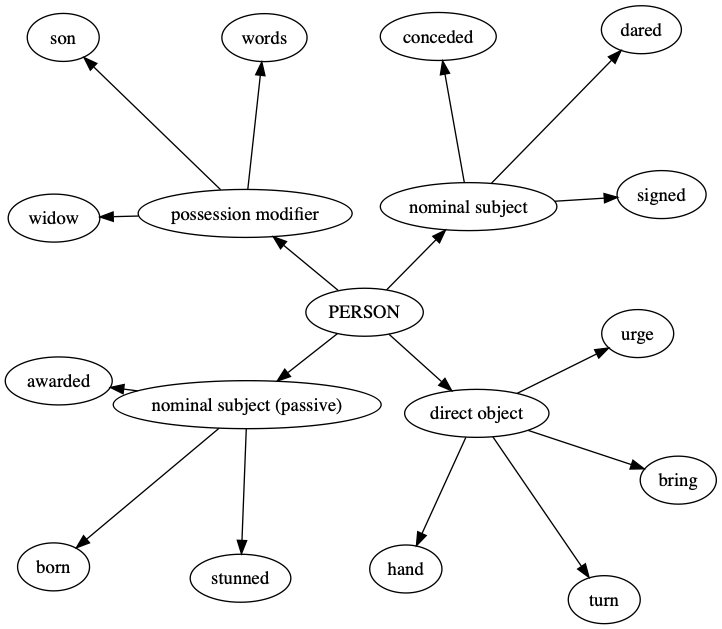
\includegraphics[width=\linewidth]{figures/G_PERSON.png}
  \caption{A simplified version of a Named Entity Type graph.}
  \label{fig:person_graph}
\end{figure}

The example in Figure \ref{fig:person_graph} shows a NET graph constructed from twelve occurrences of entities labeled as 'PERSON' in the OntoNotes corpus. We use a dependency parser to parse each sentence in which a labeled entity occurs, and we create a leaf node from the word identified by the dependency parse as the head of our labeled entity. The dependency relationship between them, which is typically labeled on the arc in a visualized dependency parse, becomes another node in between the root 'PERSON' node and its head in that occurrence.

When conducting inference, we currently rely on an existing Named Entity Recognition system to supply candidates, and our system takes over to classify the named entity type of the candidate.

For each candidate entity, we construct a graph in a similar manner to how we construct the Named Entity Template graph. The primary difference is that while we have many labeled examples of a 'PERSON' in the OntoNotes corpus, when encountering a candidate entity, we only have its one concrete occurrence. To supplement its graph, we use a coreference system to find other mentions in the text that represent the same entity, and add the relationships from each of those mentions to our graph.

We note here that while Figure \ref{fig:person_graph} shows only one generation of relationships in the direction of the dependency head, from a labeled entity to its direct head node according to a dependency parse, our NET graphs and candidate graphs actually traverse the dependency parse two generations up the tree (to the entity's head and that head's head) as well as two generations down the tree (to the entity's children, such as any adjectives modifying it, as well as the children of those children). This allows us to take in much more signal from the text that is still directly related to the entity we are considering.

Once a candidate graph has been construction, we compare it against each of our Named Entity Template graphs through a graph-similarity algorithm we developed. For our prediction we choose the label with the greatest similarity. In the case of a tie in maximum similarity scores, we choose the entity that occurs most frequently in the corpus from amidst the top scores.

We describe our process for building the graphs and computing their similarity further in Section \ref{methods}.

We think the virtue of this approach lies primarily in the transparency of the model. If desired, the system could easily be extended to include a reference point in the text for each node, for example, to point a reader to exactly which mentions in the corpus contributed to a model's interpretation.

Additionally, like any model, the more data it encounters the more robust each NET graph will become, and we believe that the interpretibility and generalizability of these graphs in describing the behavior and attributes of various entities might lead to them being utilized in other systems.

\section{Background and Related Work} \label{background}

While we ultimately decided to build a new architecture, we were informed and inspired by previous work directly related to NER as well as work from other subfields. In this section, we provide a brief survey of a few research papers and techniques and how they influenced our thinking.

\subsection{Ontology-based NER}
As our specific approach might be described as existing somewhere between Named Entity Recognition and Knowledge Representation, we considered approaches from both subfields.

We found the work of \citet{SuciuInterleavingontologybasedreasoning2014} interesting in its Ontology-based approach for logically adding labels to characters in folktales by their role within the story. And how they relate to the other characters. For example, if a boy has a parent that is a King or a Queen, then that boy is a Prince:

\begin{equation}
\resizebox{\linewidth}{!} 
  {
    $ Prince \equiv Boy \cap (\exists hasParent.King \cup \exists hasParent.Queen) $
  }
\end{equation}

We found that an intriguing concept, and wondered if we could build a system that could classify entities not just by known facts such as having a parent who is a King or Queen, but by the way they act, are acted upon, or are described.

\subsection{Transition-based NER}

Within the subfield of NER, \citet{LampleNeuralArchitecturesNamed2016} demonstrated interesting results in transition-based Named Entity Recognition. Using a similar model to a transition-based dependency parser, which processes text from left to right by considering one word at a time from a buffer of all the words in a sentence.

For each word it encounters, a traditional arc-standard transition-based system \cite{NivreIncrementalityDeterministicDependency2004} classifies the appropriate action to take from a small vocabulary of possible actions. One action in a transition-based system is a 'SHIFT' to move a word from the buffer onto a stack, which serves as both a storage area for words on which we are not yet ready to act, as well as a staging area for multi-word phrases. Another action in a typical dependency parsing transition-based system is 'REDUCE', which in arc-eager systems can come in a 'REDUCE-LEFT' and 'REDUCE-RIGHT' variety, and removes words from the buffer or stack depending on which directional variant is used, applying a dependency relation to the arc at the same time.

In this application, \citet{LampleNeuralArchitecturesNamed2016} used a similar system enhanced by Stack-LSTMs\cite{DyerTransitionBasedDependencyParsing2015} instead of simple stacks. An LSTM is a type of recurrent neural network that passes two outputs into another LSTM cell that shares its weights. One of these outputs is more directly responsive to the immediate input at each word as it moves over a text, while the other output called the 'cell state' is designed to carry signal until the chain of LSTM cells decides to alter it, thus enabling a longer 'memory' of the passage of text that has been fed through the network. The Stack-LSTMs used in this case are a hybrid of a stack data structure and a recurrent LSTM neural network designed such that each stack can maintain an embedded awareness of its full contents. And here, instead of applying dependency parse tags, their weights are trained to apply NER type labels upon a REDUCE action.

Transition-based approaches were initially designed to generate trees, and while the weights for applying labels are opaque to human interpretability, we found this method intriguing and inspiring towards our eventual approach.

\subsection{LSTMs and CRFs}

While we were particularly interested in the transition-based approach, we would be remiss in failing to discuss another architecture from the same paper\cite{LampleNeuralArchitecturesNamed2016} which had superior performance: a combination of bi-directional LSTMs and Conditional Random Fields.

In this model, the output of a pair of bi-directional LSTMs fed their output into a Conditional Random Field, which is a context-aware structure that is able to jointly model across the inputs from the sequence to capture the most likely NER tags across the sequence.

While their results of 90.46\% on the CoNLL-2003 corpus are impressive, both these results and those of the previous approach suffer from the lack of interpretability we discussed earlier, and thus we chose an alternate approach.

\section{Methods} \label {methods}

We chose to use the OntoNotes 5.0 corpus for its sizable corpus of 143,709 sentences with labeled named entities. We divided the corpus into training, dev, and test sets with a ratio of 70 / 20 / 10.

\subsection{Creating our Named Entity Type Graphs} \label{construct_net}

For each occurrence of a labeled named entity in our training set, we do the following:

1. If this occurrence of a named entity consists of more than one word (ex. 'Nobel Peace Prize'), we assume the head of the phrase to be the last word of the named entity phrase.

2. We load the graph for the Named Entity Type represented by that occurrence ('PERSON', 'ORGANIZATION', 'WORK\_OF\_ART', etc.). Using the example of 'Nobel Peace Prize', we would load the graph for its entity type: 'WORK\_OF\_ART'.

3. We look at the dependency parse of the sentence in which the entity occurrence appears, and add the entity's head token to a list, and its children token to a list. The steps below repeat for each of the words added to these lists.

4. We look at the relationship identified by the dependency parse between the root node of the graph and the head or child we are considering. If the Named Entity Type graph already has a node corresponding to that relationship, we load it as our "intermediary node" and add a one to its occurrence count. If it does not yet exist, we create it and assign it a count score of one. In the 'Nobel Peace Prize' example, we see that 'Prize' is a 'direct object' with 'awarded' as its head, so we find the 'direct object' child node of the 'WORK\_OF\_ART' root node. If there isn't already a 'direct object' node, we create it, and assign it a score count of one. If it is already there, we increase a score count by one for the ability to explore different similarity functions later on.

We chose to implement the dependency relationships as intermediary nodes rather than labels on our edges for two reasons: First, it saves us time during inference by allowing us to use graph library methods to directly access the intermediary node that represents how a given candidate entity is being used in a sentence. Additionally, it generates cleaner, more interpretable graphs, with natural clustering of the head words resulting from a particular syntactic usage of the entity type.

5. Under the intermediary node, we now add a leaf node for our named entity's head in the dependency parse. In the 'Nobel Peace Prize' example, the head of 'Prize' when it was used as a direct object is 'awarded,' so we create a node for 'awarded' as a child node of 'direct object' and give it a score of one, unless it already exists, in which case we increase its score by one.

6. In the special case of arriving at a preposition, we take an extra leap up the dependency tree to find that preposition's head, as we found more signal present in the heads of the prepositions rather than in the prepositions like "to" or "of" themselves.

7. If we were processing a head node, we add its head to our head list, and if we were processing a child node, we add its children to our child list, and we repeat the process for one more generation, with this node we have arrived at acting as the new root node of our next generation.

\subsection{Conducting Inference on a New Named Entity Candidate}

We consider each Named Entity as identified by an existing NER system\footnote{For candidate identification we used spaCy's \cite{spacy2} built-in NER module.} For each named entity candidate, we do the following:

1. We construct a candidate graph in a similar manner to that described above for generating the Named Entity Type graphs. We use a coreference system to include multiple references to the entity in order to generate as robust a graph as possible to compare against our NET graphs.

2. We compare our candidate graph to each of the eighteen Named Entity Type graphs. We only consider the subgraphs branching from intermediary nodes (the syntactic role nodes from the dependency relations) that are contained in our candidate graph, which saves us a lot of processing time on each of the extensive NET graphs.

3. Traveling down the branches of the matching intermediary nodes, we calculate a score for each successor node (the words that represent the head or child of our original node). If that successor node is a leaf node, we calculate the score directly as described below. If it has further intermediary node successors (which would be further dependency relations that match between the candidate graph and the NET graph against which we are comparing it), we travel down those branches to their leaf nodes, and eventually assign this node a score of the sum of its successors' scores.

4. For each of our candidate graph's leaf nodes, we compare that word's similarity to the similarity of all the leaf nodes under the NET's corresponding intermediary node by a comparison of their word embeddings.\footnote{This score is using spaCy's Token.similarity() method. This seems to be a cosine similarity of the words' embeddings, but it is not explicitly stated as such in their documentation.} We take the highest-scoring similarity measurement as our score for this leaf node. Concretely, if we were considering a candidate entity used as a possession modifier, and its head in that relationship (the thing it possessed) was "city," then in comparing that with the children of a Named Entity Type graph's 'possession modifier' intermediary node branching from its root, we would find that its highest-scoring successor "town" gets a rating score of 0.77 vs. another successor "missiles," which gets a score of 0.11. So in this case we would add a score of 0.77 to this branch of this Named Entity Graph's similarity score, indicating that both of these entity's may have something city-like or town-like. We tried various alternative similarity scores, which we discuss below in Section \ref{sim_scores}, but found this most basic accumulation of similarity evidence to work the best in our practice so far. 

4. We sum the scores of each "syntactic function node"'s highest-scoring child nodes to arrive at the similarity score for that Named Entity Type Graph.

5. We compare the score of each NET graph, and choose the highest-scoring type which best matched our candidate graph as our prediction. If we encounter a tie, we choose the Named Entity Type that appears most frequently in the corpus from among our top-scoring NETs.

\subsection{Trying different similarity score approaches.} \label{sim_scores}

We tried a number of approaches of formulas for best evaluating the similarity of each syntactic branch of the graph. To show the equations, we will use the following conventions:

\begin{itemize}
\item $L$ represents the NET graph's leaf node that corresponds syntactically with our candidate graph's leaf node which we are scoring, and has the highest similarity score of its sibling nodes to our candidate node.
\item $L_{count}$ represents the count of occurrences of that node
\item $Int_{count}$ represents the count of the intermediary node that is a predecessor to this node on the graph (so in the first generation of our graphs, $Int$ represents the syntactic relationship of $L$ to the entity, and $Int_{count}$ represents how many times this entity type filled that syntactic role in our training corpus)
\end{itemize}

Initially, we tried to take into account how frequently $L$ appeared in that syntactic relationship to the head node. The intuitive motivation was that while a person might 'release' a prisoner, organizations probably more commonly 'release' press releases, and thus the frequency within each syntactic branch of each NET would be indicative of how commonly used that behavior is for that type of entity.

$$ log(L_{score}) + log(\frac{L_{count}}{Int_{count}}) $$

This resulted in very poor performance (equivalent to random guessing), however, particularly on entity types such as 'PERSON' and 'ORG' which appear frequently, and therefore the matches were unduly penalized by the size of $Int_{count}$.

In order to relax the penalty of more-commonly occurring intermediary nodes, we tried this with the square root of both the count and the intermediary node count:

$$ log(L_{score}) + log(\frac{L_{\sqrt(count)}}{Int_{\sqrt(count)}}) $$

We also tried a logarithmic approach there without the outer log probabilities, as our numbers weren't too close to zero as to make those essential:

$$ L_{score} * \frac{L_{log(count)}}{Int_{log(count)}} $$

These methods improved performance on a small subset of candidates by not penalizing the more frequently occurring types as severely, but they were still penalized, and thus this method still resulted in worse performance than simply using the similarity counts on their own.

We note that by using similarity scores between word embeddings, we are potentially violating our principle of avoiding difficult-to-explain mathematical constructs. But we believe that the concept of a comparison measurement between the usage of words is explained easily enough to still be considered 'auditable', even if a lay person might not be able to generate those measurements arrived at by a cosine similarity.

\section{Results and discussion}

As we were focused on disambiguation rather than named entity chunking within this project, we measured our results on all entities where the named entity chunks we were provided by our chunking system\footnote{spaCy's NER module} matched with the labeled chunks in the OntoNotes corpus.

Table \ref{outcomes} shows our results. Naturally, we were hoping for better performance from the model than we achieved, so we will take a moment to investigate where our model worked best, and where it tended to go wrong.

\begin{table*}[ht]
\begin{tabular}{lllllll}
\toprule
Entity Type   & Precision & Recall  & F1-Score & Support  & Avg. Degree & No. Nodes \\ 
\midrule
CARDINAL      & 23.45\%   & 24.47\% & 23.95\%  & 1590     & 2.59        & 5109       \\
DATE          & 43.19\%   & 27.18\% & 33.36\%  & 2870     & 3.10        & 6078    \\
EVENT         & 1.72\%    & 8.62\%  & 2.87\%   & 116      & 1.74        & 1350   \\
FAC           & 4.14\%    & 12.08\% & 6.16\%   & 149      & 1.75        & 1739 \\
GPE           & 35.43\%   & 23.91\% & 28.55\%  & 3509     & 3.15        & 8976    \\
LANGUAGE      & 1.68\%    & 42.86\% & 3.23\%   & 7        & 1.74        & 452      \\
LAW           & 3.24\%    & 9.23\%  & 4.80\%   & 65       & 1.59        & 701 \\
LOC           & 3.65\%    & 9.76\%  & 5.32\%   & 297      & 2.00        & 2312 \\
MONEY         & 28.92\%   & 45.13\% & 35.25\%  & 822      & 2.23        & 3253     \\
NORP          & 21.27\%   & 28.49\% & 24.35\%  & 1404     & 2.40        & 5293    \\
ORDINAL       & 6.71\%    & 22.01\% & 10.28\%  & 359      & 2.01        & 1554     \\
ORG           & 44.02\%   & 19.50\% & 27.03\%  & 3867     & 2.77        & 11135    \\
PERCENT       & 20.91\%   & 16.49\% & 18.44\%  & 667      & 2.05        & 2171 \\
PERSON        & 42.58\%   & 36.80\% & 39.48\%  & 2891     & 2.60        & 9640    \\
PRODUCT       & 3.40\%    & 9.85\%  & 5.06\%   & 132      & 1.84        & 1348 \\
QUANTITY      & 3.82\%    & 9.29\%  & 5.41\%   & 183      & 1.86        & 1471 \\
TIME          & 5.30\%    & 12.44\% & 7.43\%   & 201      & 2.03        & 1478 \\
WORK\_OF\_ART & 1.67\%    & 15.87\% & 3.02\%   & 63       & 1.77        & 1743 \\ 
\midrule
Overall       & 34.04\%   & 25.62\% & 28.05\%  & 19192    & 2.18 (avg.)  & 3656 (avg.)
\end{tabular}
\caption{Our results show that our overall performance was best on 'PERSON'-type entities. We also display some metadata of each entity's NET graph.}
\label{outcomes}
\end{table*}

\subsection{Where our model succeeded}

We see that our model performed best on identifying 'PERSON' type entities according to the F1 score, and that 'PERSON' was among the top performers in terms of both precision and recall. Other top performers include 'ORG', 'GPE', 'DATE', and 'MONEY'.

In evaluating the metadata of our NET graphs, we see that all five of those NETs have among our highest average degree scores of over 2.2 in call cases (with all but 'MONEY' having an average degree of over 2.7), . By contrast, our lowest performing NET types such as 'WORK\_OF\_ART', 'EVENT', and 'LAW' all have average degree scores of $\sim$1.7 or below. We also see that our lowest performers each encountered fewer than 2,000 examples in our training set, and our top performers each encountered greater than 6,000 except for 'MONEY' which came in at a little over 3,000 nodes, but may have just been easier to classify.

We show how our performance improved with more nodes and higher average degree in Figure \ref{fig:performance}. This does suggest that our model was functional and became more accurate as it learned on more data, although improvements appear to begin tapering off in the addition of more nodes at around 5,000 nodes and in the increased average degree at around 2.4. We believe the additional features we discuss in Section \ref{enhancements} could allow for continued performance improvements as the size of our training data continued to scale.

\begin{figure*}[ht]
  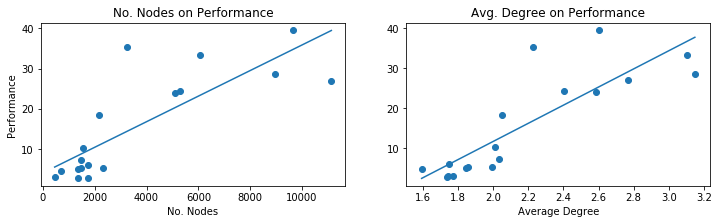
\includegraphics[width=\textwidth]{figures/performance.png}
  \caption{We see that performance improved both with more examples overall (no. of nodes) as well as greater average degree (specifically more examples per syntatic role).}
  \label{fig:performance}
\end{figure*}

\subsection{Where our model failed}

As of the obvious inverse to where we succeeded, we note that our model failed most significantly where we lacked enough training examples.

Additionally, one thing we realized early on in this approach was that nearly every other entity type is personified to an extreme degree. While a person might 'run,' so too might an organization 'run a bake sale,' and a work of art might 'run up a high price.' Therefore the verb of running is not so indicative of a 'PERSON' type as we initially believed. In fact, it is difficult to conceive of a verb or adjective indicative of one class that could not be utilized by other entity types as well.

Another limitation of our model was the time it took to generate the NET graphs and evaluate the documents of our dev set. While we adjusted our architecture to parallel computations across a cluster in order to improve this time, it still took > 18 hours for all jobs to finish accross a Kubernetes cluster of 26 nodes with a combined 52 vCPUs and 195GB RAM. We expected this approach to not be the most speed-optimized technique given the graph-based approach rather than a vectorized approach taking advantage of matrix multiplication, but it made iteration and experimentation slower than anticipated.

\subsection{Possible enhancements} \label{enhancements}

Ideas for possible enhancements include:

\begin{itemize}

\item If it appears we are filtering out too much signal by being too selective, we are considering adding a hyperparameter that would not just take the immediate head and children of each entity in our NET graphs and inference candidates, but take one or two additional generations of head and child nodes, if they exist. This might allow us to take in more information while still filtering out noise that doesn't have a directly traceable dependency relation to the entity in question.

\item If inference is too slow due to the large size of the NET graphs, we have considered compressing the information in those graphs by clustering the leaf nodes using a Partitioning Around Medoids algorithm to find the 50 or so most representative leaf nodes and having those absorb the weights of the other members in their cluster, which we could then discard. We think this would serve as a sort of regularization to allow the model to accept more synonyms rather than exact matches of candidate entity's head to leaf nodes, while still maintaining the clarity of having real word leaf nodes.

\item Add the children of our head to capture direct objects of the verb.

\item Alternatively, if the model is too sensitive to whether a candidate entity's head matches exactly to a leaf node in our NET graphs, we could do clustering of the leaf node words via k-means, such that our clusters' centers would \textit{not} be actual words, but would exist somewhere in the embedding space near the words, and thus no word would likely be a 100\% match. To maintain interpretability, we could maintain a list of the closest leaf node to each cluster center.

\item We considered giving each syntactic function node a trainable weight, and then training those weights via a logistic regression type neural network to emphasize or deemphasize the importance of certain syntactic functions for classifying certain Named Entity Types, but we don't expect the candidate graphs to have enough different syntactic functions represented to make this worthwhile.

\item We posit that running a TF-IDF weighting of the leaf nodes would improve results by bringing out the most salient examples in each graph.

\item Another potential method we predict would improve the accuracy of our model is to replace certain types of strings with a common replacement. For example, we would replace digits with '11', dates of all formats with '11/11/1111', and percentages with '99\%.' This replacement would be made in the NET graphs as well as in the candidate graphs. By reducing the large variance in numerical representations, we would be able to provide more accurate probabilities surrounding those tokens.

\item Lastly, we are considering pruning stop words from the NET graphs, again in hopes of removing noise from the model.

\end{itemize}

\section{Conclusion}

Given more time to improve the inference performance of the model and to improve the features and weights included in the graph model, we believe this system could develop into a powerful classifier for longer literary works such as novels.

In addition to being useful for interpretable Named Entity Disambiguation, the Named Entity Type graphs are interesting artifacts themselves, and we see additional possible uses for these techniques. One example use case might be in creating graphs that model the portrayal of different characters in a novel, for example, perhaps with a different graph for each chapter to help publishers and authors plot the development of characters over a longer work.

With additional refinement and the appropriate labeled dataset, we could classify a protagonist in a novel as a traditional hero or an anti-hero. We could identify occupations or literary tropes represented by supporting characters. And interesting tools for authors or publishers could be developed by tracking changes in a character's behavior from heroic to antiheroic from chapter to chapter.\cite{LampleNeuralArchitecturesNamed2016}

Furthermore, we see the potential of graph-based 'mental constructs' as having additional applications in the progression of machine learning. We believe transition-based parsing approaches could directly build on these graphs, and logical operations could be conducted on them to build out unstated but implied nodes that enhance our understanding of entities beyond what is explicitly stated. \cite{NivreIncrementalityDeterministicDependency2004}

% include your own bib file like this:
%\bibliographystyle{acl}
%\bibliography{acl2018}
\bibliography{acl2018}
\bibliographystyle{acl_natbib}

\end{document}
